
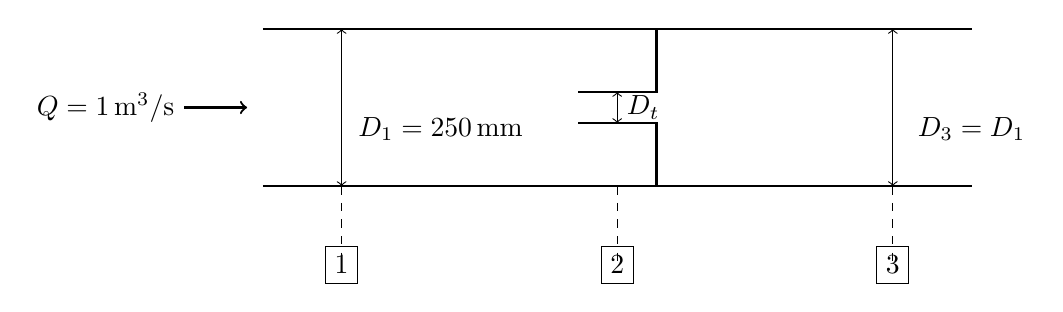
\begin{tikzpicture}
    % Draw the pipes
    \draw[thick] (-1, 1) -- (8, 1); % upper pipe
    \draw[thick] (-1, -1) -- (8, -1); % lower pipe

    % Draw flow rate arrow and label
    \draw[->, thick] (-2, 0) -- (-1.2, 0);
    \node[left] at (-2, 0) {$Q = 1 \, \mathrm{m^3/s}$};

    % Draw diameter lines and labels
    \draw[<->] (0, 1) -- (0, -1);
    \node[below] at (1.256, 0) {$D_1 = 250 \, \mathrm{mm}$};
    
    % Draw two small boxes for the middle section
    \draw[thick] (4, -1) --(4, -0.2)--(3,-0.2); % bottom box
    \draw[thick](4, 1) --(4, 0.2)--(3,0.2);   % top box

    % Draw diameter line between boxes and label
    \draw[<->] (3.5, 0.2) -- (3.5, -0.2);
    \node[right] at (3.5, 0) {$D_t$};

    % Draw diameter line and label on the right
    \draw[<->] (7, 1) -- (7, -1);
    \node[below] at (8, 0) {$D_3 = D_1$};

    % Draw the measurement points
    \node[draw, rectangle] at (0, -2) {1};
    \draw[dashed] (0, -1) -- (0, -2);

    \node[draw, rectangle] at (3.5, -2) {2};
    \draw[dashed] (3.5, -1) -- (3.5, -2);

    \node[draw, rectangle] at (7, -2) {3};
    \draw[dashed] (7, -1) -- (7, -2);
\end{tikzpicture}

